%!TEX encoding = UTF-8 Unicode

%!TEX root = ../compendium.tex

\Lab{\LabWeekEIGHT}

\begin{Goals}
\item Kunna använda mönstermatchning
\item Känna till exceptions
\item Förstå hur Try fungerar

\end{Goals}

\begin{Preparations}
\item Gör övning {\tt \ExeWeekEIGHT} i kapitel \ref{exe:W08}.
\item Läs om exceptions och felhantering.
\item Bonus: ha tillgång till en dator där ni kan spela upp ljud.
\end{Preparations}

\subsection{Bakgrund}
Inom musik utgår man från en skala med 12 olika toner (C, C\#, D, D\#, E, F, F\#,G, G\#, A, A\#, B). Nästa ton efter B är C och tillhör nästa oktav. Ett ackord är uppbyggt av ett antal olika toner som spelas tillsammans. Laborationen kommer att utgå från två olika instrumant: gitarr och ukulele. Skillnaden för dessa två instrument är antalet strängar och vilken tonart de är stämda i. På båda instrumenten har en grepbräda med ett antal olika band. Ett ackord spelas genom att man med ett finger trycker ner på strängen på band $i$. Om strängen spelas kommer tonen att vara ett halvt tonsteg högre än om man håller ner strängen på plats $i-1$.

Laborationen kommer bestå av ett textbaserat användargränssnitt där man kommer ha möjlighet bl.a. att lägga till nya ackord, rita upp ackord och spela ackord. En ton anges på följande format "E2", vilket innebär andra oktaven tonen E. Rekommenderad stämning för gitarr resp. ukulele är: E2, A2, D3, G3, B3, E4 resp. G4, C4, E4, A4. Denna stämning kommer fungera för de fördefinierad ackorden i filen chords.txt.

Om ni är fler än fyra i gruppen behöver ni även göra extrauppgiften, men om ni däremot är enbart tre behöver ni inte implementera play.

\subsection{Obligatoriska uppgifter}

\Task \code{Notes}. Objektet ska kunna omvandla en tons namn (t.ex. "E2") till
en heltalsrepresentation och tvärtom.

\Subtask Implementera först metoden \code{fromNbrToNote} med hjälp av \code{%}-operatorn


\Subtask Implementera metoden \code{unapply} som ska ta in en sträng (t.ex. "E2") och tonens nummer. "E2"\ kommer översättas till 16 och "C1"\ till 0 och tänk på att hantera specialfallet då till exempel "C\#1"\ ska ge värdet 1. Använd attributet \code{toNumber} för att översätta en ton utan oktav ("C\#", "E") till ett nummer. Titta gärna på vad metoden \code{zipWithIndex.toMap} gör och använd den i \code{toNumber}.

\Subtask Använd \code{TestNotes} som ligger i paketet \code{test} för att se till så att \code{Notes} är rätt implemeterat. Starta \code{TestNotes} och rätta till eventuella fel.

\Task \code{Chord}. Representation av de två olika ackorden. Lägga märken till
hur stämning (eng. \textit{tuning}) och ett grepp (eng. \textit{grip}) representeras i \code{Chord}. $-1$ i ett grep betyder att strängen inte ska
spelas.

\Subtask Implementera \code{toString} så att den matchar utskriften i filen \textit{chords.txt}. I objektet \code{Chord} ska \code{toString} vara på formen
D:-1 -1 0 2 3 2

\Subtask Implementera metoden \code{isIncludedBy}.  Använd \code{.split(";")} för att dela upp strängen \code{filter} i de olika filtersträngarna. Kolla för varje filtersträng om den includeras i \code{toString}. Exempel på filtersträng: "git:G;B;uku". \textbf{Tänk på att metoden \code{forall} kollar om ett villkor gäller för alla möjligheter. I det här fallet räcker det att det gäller för ett av fallen}

\Subtask Implementera \code{isGit} och \code{isUku} som jämför början av strängen \code{s} och returnerar \code{true} om strängen matcher ett gitarrackord resp. ukuleleackord.

\Subtask Implementera klassen \code{Guitar}. \code{toString} ska vara på samma format som i filen \textit{chords.txt}.

\Subtask Skapa en ny klass \code{Ukulele} som har liknande beteende som \code{Guitar}.

\Subtask Implemetera \code{instToChord} med hjälp av \code{matching} och låt basfallet (om ackordet är varken gitarrackord eller ukuleleackord) retunera \code{None}.

\Task \code{database}. Kommer hålla reda på alla ackord i programmet. Testa varje metod innan nästa blir implemeterad. Det blir då lättare att upptäcka fel i koden.

\Subtask Börja med att implemetera \code{add} och \code{allChords}.

\Subtask Implementera \code{find} och \code{updateFilter}. \code{find} ska inte retunera enbart den första förkomsten av söksträngen utan alla. Metoden \code{find} i \code{Vector} retunerar enbart första förekomsten.

\Subtask Implementera \code{filteredChords} och \code{sort} med hjälp av metoden \code{isIncludedBy} i \code{Chord}. Tom filtersträng innebär att inget filter appliceras. Vid \code{sort} kan man ta hjälp av metoden \code{sortBy} i \code{Vector}.

\Subtask Implementera \code{delete}. \textbf{Tänk på att \code{delete} ska radera ackordet på plats $i$ i \code{filteredChords} och inte i code{allChords}}

\Task textui

\Subtask Provkör programmet och prova några olika kommandon (t.ex. add, del, help). Använd metoderna i \code{database} för att implementera kommandona.

\Subtask Titta på objektet \code{Help}. Använd liknande \code{matchning} för att ta hand om alla fall för de olika kommandona.

\begin{itemize}
\item \code{Add}. Argumenten måste först bli en sträng med hjälp av \code{mkString(" ")} för att sedan delas upp vid ';'. Användaren kan skriva in felaktiga ackord, vilket måste hanteras. Metoden \code{fromString} i \code{Chord} retunerar ett \code{Option[Chord]}. Titta närmare på metoden \code{flatMap}.

\item \code{Lst}. Använd \code{matching} för att ta hand om fallet när användaren anger argument till kommandot, vilket inte ska vara med. Använd metoden i \code{database}. Listan ska vara numrerad från $1$.

\item \code{Del}. Använd \code{matching} för att ta hand om felfallen inget arguement och fler än ett argument. Ett tredje felfall är om användaren anger något annat än en siffra som argument. Använd \code{Try} och \code{matching} för att ta hand om felet.

\item \code{Filter}. Använd metoderna i \code{database}. De filtrerade ackorden behöver inte skrivas ut efter filtrering, utan användaren behöver använda kommandot \code{list} för att lista de filtrerade ackorden.

\item \code{Find}. Använd \code{matching} för att ta hand om felfallen inget argument eller fler än ett argument.

\item \code{Load}. Använd \code{matching} för att ta hand om felfallen inget argument eller fler än ett argument. Använd metoden \code{load} i objektet \code{io} för att läsa in från den angivna filen. Metoden kommer likna metoden \code{Add}.

\item \code{Save}. Använd \code{matching} för att ta hand om felfallen inget argument eller fler än ett argument. Använd metoden \code{save} i objektet \code{io} för att skriva till den angivna filen. Om filen inte finns kommer den skapas.

\item \code{Sort}. Använd \code{matching} för att ta hand om fallet när användaren anger arguement till kommandot, vilket inte behövs. Använd metoden i \code{database}.

\item \code{Quit}. Använd \code{matching} för att ta hand om fallet när användaren anger arguement till kommandot, vilket inte behövs. Skapa en hjälpmetod \code{quitPrompt} som returnerar en \code{Boolean} med värdet \code{true} om användaren anger 'y', \code{False} om användaren anger 'n' och som körs igen vi felaktigt svar (allt annat än 'y' och 'n'). Även 'Y' och 'N' ska vara acceptabelt svar.

\item \code{Play}. Använd \code{matching} för att bryta ut de olika argumenten och för att ta hand om felfallet inga argument. Första argumentet är tempo i millisekunder och resten är siffror som motsvarar platsen för ackordet i den filtrerade listan. Varje sträng i argumentlistan ska omvandlas till \code{Int} och det är viktigt att ta hand om fallet då användaren anger något annat än en siffra. Använd \code{Try} och \code{matching} för att ta hand om felet. Använd \code{ChordPlayer} för att spela upp ett ackord. \textbf{Kom ihåg att lägga till kommandot i listan med kommandon i \code{doCommand}}

\item \code{Draw}. Använd \code{matching} för att ta hand om felfallen inget argument eller fler än ett argument. Argumentet motsvarar ackordets plats i den filtrerade litan. Använd \code{Try} och \code{matching} för att ta hand om felet att användaren anger något annat än en siffra. Använd \code{ChordDraw} för att rita upp ackord. \textbf{Kom ihåg att lägga till kommandot i listan med kommandon i \code{doCommand}}
\end{itemize}

\Task \code{ChordPlayer}. Ska spela upp enstaka ackord \code{chord} med en viss längd \code{time} i millisekunder.

\Subtask Titta vilka parametrar metoden \code{play} i \code{SimpleNotePlayer} behöver. Heltalet \code{note} ska vara heltalsrepresentationen av en ton.

\Subtask För att omvandla ett ackord till toner behöver först stämningen, \code{tuning}, omvandlas till sin heltalsrepresentation och sen ska greppet, \code{grip}, adderas till stämningen för varje sträng. Varje strängs ton ska sedan spelas upp under den angivna tiden. Koden för att spela ackordet ska placeras ovanför den existerande koden. \textbf{Tänk på att strängar med greppet -1 inte ska spelas}

\Subtask Skapa ett nytt kommando i \code{textui} som heter \textit{play}. Se instruktioner för \code{textui}.

\subsection{Extrauppgifter}

\Task ChordDraw

\Subtask Rita upp en greppbräda liknande bilden nedan (kryssen läggs till i kommande uppgifter). Antalet strängar ska variera beroende på instrument.

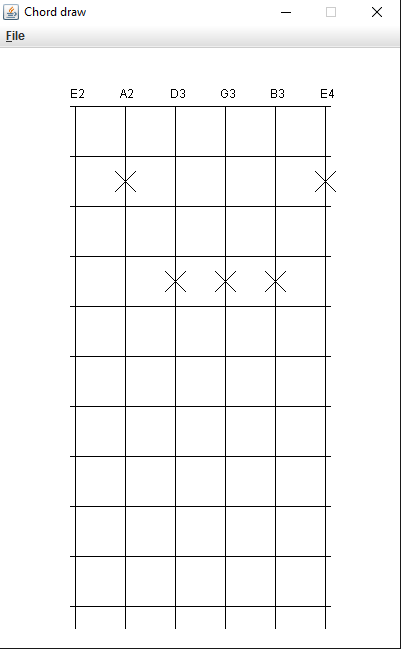
\includegraphics[width=0.5\textwidth]{../img/chords/ChordDraw}

\Subtask Skapa en hjälpmetod \code{cross} som tar in två heltal $x$ och $y$. Metoden ska rita upp ett kryss som är 20x20 pixlar och har sitt centrum i en angivna koordinaten.

\Subtask Rita ut ett kryss där en sträng trycks ner. \textbf{Tänk på att -1 och 0 anger att en sträng inte trycks ner}.

\Subtask Implementera metoden \code{play} som börjar med att vänta på ett event från \code{SimpleWindow}, sedan kollar om eventet är av typen \code{SimpleWindow.MOUSE_EVENT}. Sedan ska man kolla om användaren trycket på någon sträng (ett intervall på -10 till +10 i förhållande till strängens x-koordinat kan anses vara på strängen). Om användaren tryckt på en sträng ska denna spelas med hjälp av \code{SimpleNotePlayer}. Metoden \code{play} ska köras tills användaren kryssar ner fönstret, vilket motsvarar \code{SimpleWindow.CLOSE_EVENT}.

\Subtask Skapa ett nytt kommando i \code{textui} som heter \textit{draw}. Se instruktioner för \code{textui}.